%%%%%%%%%%%%%%%%%%%%%%%%%%%%%%%%%%%%%%%%%%%%%%%%%%%%%%%%%%%%%%%%%%%%
%% I, the copyright holder of this work, release this work into the
%% public domain. This applies worldwide. In some countries this may
%% not be legally possible; if so: I grant anyone the right to use
%% this work for any purpose, without any conditions, unless such
%% conditions are required by law.
%%%%%%%%%%%%%%%%%%%%%%%%%%%%%%%%%%%%%%%%%%%%%%%%%%%%%%%%%%%%%%%%%%%%

\documentclass[
  digital, %% This option enables the default options for the
           %% digital version of a document. Replace with `printed`
           %% to enable the default options for the printed version
           %% of a document.
  twoside, %% This option enables double-sided typesetting. Use at
           %% least 120 g/m² paper to prevent show-through. Replace
           %% with `oneside` to use one-sided typesetting; use only
           %% if you don’t have access to a double-sided printer,
           %% or if one-sided typesetting is a formal requirement
           %% at your faculty.
  notable,   %% This option causes the coloring of tables. Replace
           %% with `notable` to restore plain LaTeX tables.
  nolof,   %% This option prints the List of Figures. Replace with
           %% `nolof` to hide the List of Figures.
  nolot,   %% This option prints the List of Tables. Replace with
           %% `nolot` to hide the List of Tables.
  %% More options are listed in the user guide at
  %% <http://mirrors.ctan.org/macros/latex/contrib/fithesis/guide/mu/fi.pdf>.
]{fithesis3}
%% The following section sets up the locales used in the thesis.
\usepackage[resetfonts]{cmap} %% We need to load the T2A font encoding
\usepackage[T1,T2A]{fontenc}  %% to use the Cyrillic fonts with Russian texts.
\usepackage[
  main=slovak,  %% By using `czech` or `slovak` as the main locale
                %% instead of `english`, you can typeset the thesis
                %% in either Czech or Slovak, respectively.
  %english, german, russian, czech, slovak %% The additional keys allow
]{babel}        %% foreign texts to be typeset as follows:
%%
%%   \begin{otherlanguage}{german}  ... \end{otherlanguage}
%%   \begin{otherlanguage}{russian} ... \end{otherlanguage}
%%   \begin{otherlanguage}{czech}   ... \end{otherlanguage}
%%   \begin{otherlanguage}{slovak}  ... \end{otherlanguage}
%%
%% For non-Latin scripts, it may be necessary to load additional
%% fonts:
\usepackage{paratype}
\def\textrussian#1{{\usefont{T2A}{PTSerif-TLF}{m}{rm}#1}}
%%
%% The following section sets up the metadata of the thesis.
\thesissetup{
    date          = \the\year/\the\month/\the\day,
    university    = mu,
    faculty       = fi,
    type          = mgr,
    author        = Bc. Ondrej Oravčok,
    gender        = m,
    advisor       = {RNDr. Radek Ošlejšek, Ph.D.},
    title         = {Interaktívna časová os ako modul v Angulare},
    %TeXtitle      = {The Proof of $\mathsf{P}=\mathsf{NP}$},
    TeXtitle      = {Interaktívna časová os ako modul v Angulare},
    keywords      = {keyword1, keyword2, ...},
    TeXkeywords   = {keyword1, keyword2, \ldots},
    abstract      = {This is the abstract of my thesis, which can

                     span multiple paragraphs.},
    thanks        = {These are the acknowledgements for my thesis, which can

                     span multiple paragraphs.},
    %bib           = prace.bib,
}
\usepackage{makeidx}      %% The `makeidx` package contains
\makeindex                %% helper commands for index typesetting.
%% These additional packages are used within the document:
\usepackage{paralist} %% Compact list environments
\usepackage{amsmath}  %% Mathematics
\usepackage{amsthm}
\usepackage{amsfonts}
\usepackage{url}      %% Hyperlinks
\usepackage{markdown} %% Lightweight markup
\usepackage{listings} %% Source code highlighting
\usepackage{xcolor}
\definecolor{_blue}{RGB}{0,0,184}
\definecolor{_green}{RGB}{60,128,49}
\definecolor{_gold}{RGB}{153,122,26}
\definecolor{_purple}{RGB}{121,0,196}
\lstdefinelanguage{TypeScript}{
    keywords = [3]{selector, templateUrl, user, subscription\$, _userService, console},
    keywords = [2]{@Component, ngOnInit, ngOnDestroy, unsubscribe, subscribe, log},
    keywords = [1]{number, string, object, typeof, let, public, private, void, this, implements, export, class, constructor },
    sensitive=true, % keywords are not case-sensitive
    morecomment=[l]{//}, % l is for line comment
    morecomment=[s]{/*}{*/}, % s is for start and end delimiter
    morestring=[b]' % defines that strings are enclosed in double quotes
}
\lstset{
%  basicstyle      = \ttfamily,%
%  identifierstyle = \color{black},%
%  keywordstyle    = \color{blue},%
%  keywordstyle    = {[2]\color{cyan}},%
%  keywordstyle    = {[3]\color{olive}},%
%  stringstyle     = \color{teal},%
%  commentstyle    = \itshape\color{magenta}}
  language=TypeScript,
  aboveskip=3mm,
  belowskip=3mm,
  showstringspaces=false,
  columns=flexible,
  basicstyle={\small\ttfamily},
  numbers=left,
  xleftmargin=1.25em,
  numberstyle=\tiny\color{gray},
  keywordstyle=[3]\color{_purple},
  keywordstyle=[1]\color{_blue},
  keywordstyle=[2]\color{_gold},
  commentstyle=\color{darkgray},
  stringstyle=\color{_green},
  breaklines=true,
  escapeinside={<@}{@>},
  showlines=true,
%  breakatwhitespace=true,
%  tabsize=3
}
\renewcommand{\lstlistingname}{Ukážka}% Listing
\renewcommand{\lstlistlistingname}{List of \lstlistingname s}% List of Listings
\usepackage{floatrow} %% Putting captions above tables
%\floatsetup[table]{capposition=top}
\usepackage[backend=biber,sorting=none]{biblatex}
\addbibresource{prace_mgr.bib}
\usepackage{graphicx}
\graphicspath{ {pics/} }
\usepackage{tabu}
\usepackage{multirow}

\newtheorem{mydef}{Definícia}
\def \angular_version {5.2.10}

\begin{document}
\chapter*{Úvod}
\addcontentsline{toc}{chapter}{Introduction}
Toto bude úvod.

\chapter{Kybernetický polygón}
Podľa Národného bezbečnostného úradu Českej republiky je termínom \textit{kritická informačná infraštruktúra} označený \textit{"systém prvkov tejto infraštruktúry, ktorý pri narušení svojej funkcie môže spôsobiť poškodenie alebo ohrozenie záujmov Českej republiky"}\cite{nbu2012}.

Kybernetický polygón (KYPO) bol zriadený Ministerstvom vnútra Českej republiky za účelom zaistenia kybernetickej bezpečnosti v Českej republike ochranou kritickej informačnej infraštruktúry. Projekt KYPO poskytuje unikátne prostredie pre výskum nových metód, ktoré by v blízkej budúcnosti mohli pomôcť chrániť kritickú informačnú infraštruktúru\cite{dankovvcikova2015konfigurace}. Objekt polygónu bol vybudovaný v roku 2015 vrámci rekonštrukcie Fakulty Informatiky.
%V rýchlo sa rozvíjajúcom svete informačných technológií je informačná bezpečnosť najdôležitejším odvetvím informatiky. V dnešnej dobe už nie je veľmi pravdepodobné, aby nás výdobytky techniky ako telefóny a počítače ohrozovali na živote. Hrozba informačnej bezpečnosti sa týka hlavne ochrany informácií. Masarykova Univerzita si uvedomuje vážnosť tejto hrozby a preto sa rozhodla zriadiť výzkumné stredisko v tejto oblasti.

\section{Technológie}
Prostredie KYPO funguje na princípe cloudového riešenia v ktorom je možné modelovať virtuálnu sieť\cite{eichler2014analytical}. Toto riešenie poskytuje všetky nástroje potrebné k simulácii rôznych sieťových topológií. Prostredie je určené pre výzkum a testovanie rôznych scenárov kybernetických útokov v izolovanom a plne kontrolovateľnom prostredí\cite{vceleda2015kypo}.

Spektrum kybernetických hrozieb vo svete informačných systémov je veľmi široké a každá hrozba má iný spôsob, ktorým narúša kontinuitu iného systému. Medzi časté experimenty vykonávané vrámci KYPO stoja za zmienku DDoS útoky (distributed denial of service), útoky botnet alebo phishing\cite{vcegan2014navrh, celeda2013projekt}.

\section{Architektúra}
\begin{figure}
	\center
	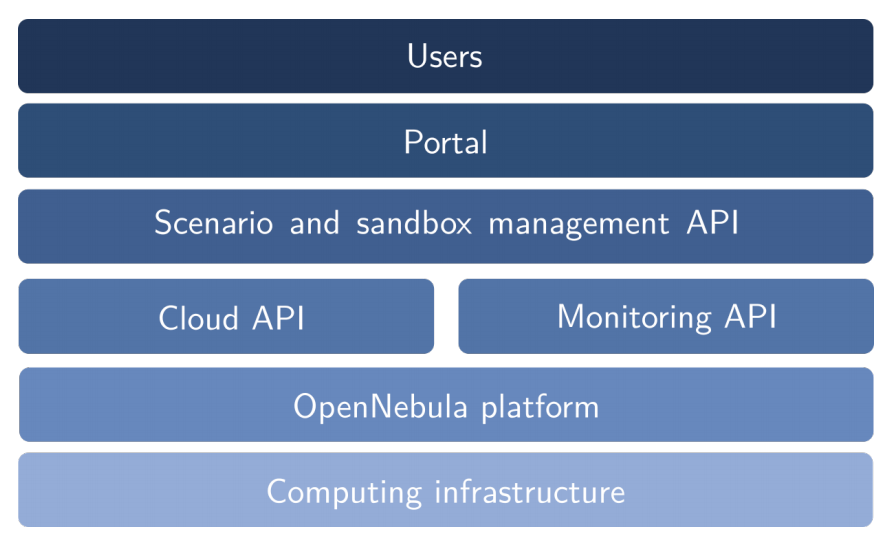
\includegraphics[width=1.0\linewidth]{kypo_structure}
	\caption{Architektúra cloudového riešenia KYPO\cite{vceleda2015kypo}}
	\label{kypo_structure}
\end{figure}

Prostredie kybernetického polygónu je implementované ako cloudové riešenie modelu Platform as a Service. Obrázok \ref{kypo_structure} znázorňuje jednotlivé vrstvy architektúry:

\begin{description}
\item[Users] - užívatelia s rôznymi skúsenosťami interagujú so systémom buď cez Portál, alebo priamo s niektorou nižšou vrstvou
\item[Portal] - Portál je grafické používateľské rozhranie (GUI), ktoré v prípade KYPO využíva portálový server Liferay opísaný v kapitole~\ref{liferay}. Praktická časť tejto práce sa zaoberá tvorbou portletu práve do tejto vrstvy architektúry.
\item[Scenario and sandbox management API] slúži na konfiguráciu, vytváranie, editovanie a likvidáciu sandboxov. Sandbox je izolovaný súbor virtuálnych strojov a sieťovej konfigurácie, ktorý užívateľovi poskytuje kľúčovú funkcionalitu ako napríklad možnosť opakovať a modifikovať experiment v prostredí KYPO.
\item[Monitoring API] umožňuje monitorovanie sieťových prepojení a konfigurácie uzlov. Komunikuje buď s OpenNebula alebo priamo s existujúcimi virtuálnymi inštanciami.
\item[Cloud API] slúži ako univerzálne rozhranie pre vyššie vrstvy ktoré abstrahuje od konkrétnej implementácie IaaS\footnote{Infrastructure as a Service} nižších vrstiev, aby bola zabezpečená flexibilita cloudového riešenia.
\item[OpenNebula platform] implementuje IaaS\cite{sempolinski2010comparison}. Umožňuje manažment rôznorodých výpočtových kapacít (najčastejšie virtualizovaných) a spadá pod správu CERIT Scientific Cloud.
\item[Computing infrastructure] zahrňuje fyzické objekty, sieťové prvky a všetok potrebný hardvér, ktorý poskytuje pamäť a výpočtovú silu.
\end{description}

\section{Logická štruktúra}
Túto štruktúru nám približuje obrázok \ref{kypo_logic_structure}.

\subsection{Bezpečnostný scenár}
Každý experiment, ktorý sa vykonáva v prostredí KYPO, je popísaný \textit{Bezpečnostným scenárom}. Bezpečnostný scenár (Security scenario) je možné prirovnať k filmovému scenáru. Sú v ňom opísaní všetci účastníci, ich úloha v danom experimente, topológia siete, úlohy jednotlivých uzlov v sieti, priepustnosť siete ale napríklad aj naplánované udalosti, ktoré nastanú v presnom čase\cite{eichler2014analytical, eichler2015kypo}.

Najčastejše bezpečnostné scenáre ako DDoS útoky, phishing alebo jednoduché hekovacie hry sú v KYPO preddefinované. Scenáre sa ukladajú vo formáte JSON\cite{eichler2015kypo}.

\begin{figure}
	\center
	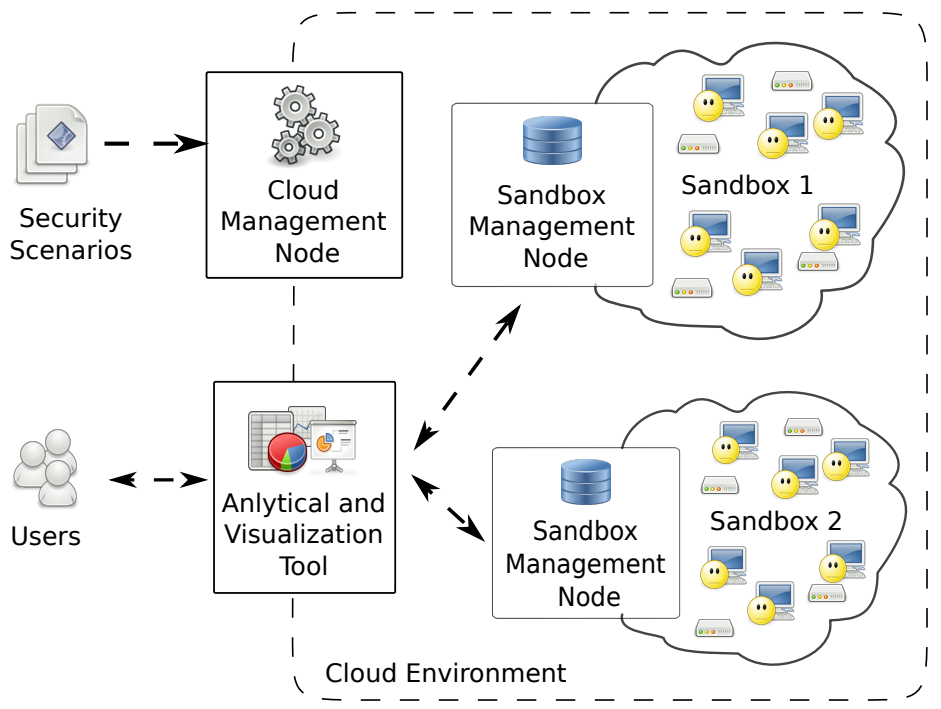
\includegraphics[width=0.875\linewidth]{kypo_logic_structure}
	\caption{Logická štruktúra KYPO\cite{eichler2015kypo}}
	\label{kypo_logic_structure}
\end{figure}

\subsection{Manažment cloudu}
Cloud Management Node (CMN) je samostatný centrálny uzol v systéme, ktorý je zodpovedný za automatickú inicializáciu sandboxov a ich manažment. CMN spracuje bezpečnostný scenár a postará sa o získanie zdrojov v cloude. Podľa popisu v bezpečnostnom scenári vytvorí jeden až niekoľko sandboxov, čo v závislosti od náročnosti môže trvať niekoľko minút až hodín\cite{eichler2015kypo}.

\subsection{Manažment sandboxov}
\label{smn}
Všetky činnosti vykonávané vrámci sandboxu, ako napríklad prenosy dát v sieti, vyťaženie procesorov alebo iné dôležité udalosti, sú monitorované, pričom o ukladanie týchto zaznamenaných hodnôt sa stará Sandbox Management Node (SMN). Každý sandbox má priradený vlastný SMN, ktorý zaznamenáva činnosť v danom sandboxe a zároveň plní funkciu akejsi vstupnej brány do prostredia sandboxu\cite{eichler2014analytical}.

Dáta, ktoré zaznamenáva SMN sú práve tie dáta, ktoré sa zobrazujú v portletoch portálu Liferay. Ten z pohľadu logickej štruktúry (na Obr. \ref{kypo_logic_structure}) spadá pod Analytical and Visualization Tool (AVT).

\section{Potreba analýzy dát}
Nakoľko simulácie útokov a cvičenia prebiehajú v reálnom čase, vznikla potreba sledovať zmeny v týchto dynamických prostrediach. Priebehy jednotlivých scenárov sa zaznamenávajú aj pre potreby neskoršej analýzy. O túto činnosť sa stará manažment sandboxov (SMN), ktorý sme si opísali v podkapitole \ref{smn} \nameref{smn}.

Portlet časovej osy slúži ako kľúčový element pre filtrovanie týchto dát, či už sa jedná o analýzu starších dát, alebo sledovanie aktuálne pribúdajúcich dát počas práve prebiehajúceho experimentu.

\chapter{Liferay Portal}
\label{liferay}
V kontexte webových aplikácií môžeme portál definovať \cite{sezov2011liferay} ako \textit{"Samostatne oddelené webové prostredie, z ktorého sú spustiteľné všetky aplikácie užívateľa. Tieto aplikácie sú systematicky integrované na jednom mieste."}

Liferay je portálový server, v ktorom je zmysluplne umožnená spolupráca a zdieľanie informácií rôznym používateľom. Umožňuje vykonávať správu obsahu pomocou WYSIWYG\footnote{WYSIWYG - \textit{what you see is what you get}, teda \textit{"to, čo vidíš je to, čo aj dostaneš"} je intuitívny spôsob vytvárania kódu v 2D grafickom prostredí, pri ktorom sa kód (najčastejšie HTML) generuje bezprostredne na základe našich pokynov. S výslednými elementami pracujeme priamo a kód sa generuje priebežne \cite{guo2011wysiwyg}.} editora. Používateľ tak nepotrebuje žiadnu hlbokú znalosť HTML ani iného programovacieho jazyka. Jednotlivé komponenty stránky si vie jednoducho prispôsobiť a výsledok vidí vždy okamžite \cite{sezov2011liferay}.

Portálový server Liferay je naprogramovaný v jazyku Java a distribuovaný pod licenciou LGPL. Na jeho beh potrebujeme aplikačný server, alebo aspoň servlet kontajner. Liferay natívne podporuje napríklad Apache Tomcat, GlassFish, JBoss, WebLogic, WebSphere a mnoho ďalších.

\section{Štruktúra}
Liferay Portal umožňuje spravovať užívateľov a priraďovať im oprávnenia na jednotlivé časti portálu, alebo ich zaraďovať do rôznych typov skupín podľa oprávnení alebo záujmov. Nasledujúce podkapitoly stručne opisujú veľmi široké možnosti Liferay portálu.

\subsection{Používatelia}
\label{liferay_users}
Do portálov majú prístup užívatelia (Users), ktorý môžu byť priraďovaný do skupín (User Groups). Užívatelia taktiež môžu byť priraďovaný do organizácií (Organizations). Tieto organizácie sú zoskupované do rôznych hierarchických štruktúr, popri ktorých ešte v Liferay existujú komunity (Communities) a tímy (Teams). Detailnejší náhľad do štruktúry nám poskytne obrázok \ref{liferay_structure}.

Liferay tak v tomto smere poskytuje pre portálových administrátorov veľmi silný nástroj a taktiež obrovskú škálovateľnosť. Informácie o jednotlivých povoleniach (Permissions) vrámci systému sú pevne definované v rolách (Roles). Užívatelia, skupiny užívateľov, organizácie a komunity môžu byť priraďované do rolí \cite{sezov2010portal}.

\begin{figure}[H]
	\center
	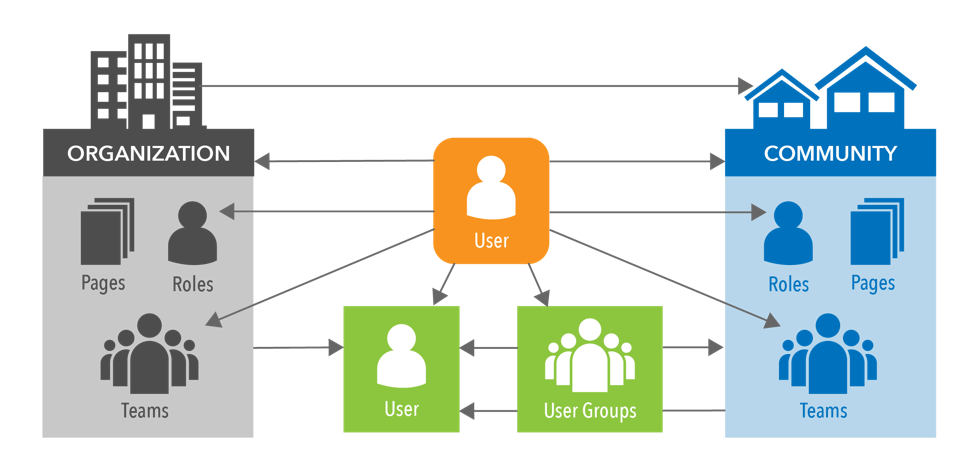
\includegraphics[width=1.0\linewidth]{liferay_structure}
	\caption{Model štruktúry a oprávnení portálového servera Liferay \cite{sezov2010portal}}
	\label{liferay_structure}
\end{figure}

\subsection{Portlety}
\label{portlets}
Základnou stavebnou jednotkou portálu v Liferay je portlet. Každá stránka portálu sa skladá z portletov, pričom každý portlet je v kontexte Liferay samostatná aplikácia. Užívateľ je schopný umiestňovať tieto portlety ľubovoľne po stránke a nastavovať im parametre.

Liferay obsahuje veľké množstvo vopred pripravených portletov, avšak jeho hlavná výhoda tkvie v možnosti rozšíriť ponuku týchto portletov o svoje vlastné. Jednotlivé stránky obsahujúce portlety (pages) je potom možné zaraďovať do lokalít (sites).

\subsection{Stránky}
Stránky sú stavebné elementy v Liferay ktoré obsahujú portlety. Podľa viditeľnosti stránok pre používateľov delíme stránky na:
\begin{description}
\item[Verejné stránky] - sú viditeľné aj pre užívateľov, ktorí nie sú registrovaný v systéme
\item[Privátne stránky] - vyžadujú sa určité oprávnenia, ktoré musí mať užívateľ priradené
\begin{itemize}
\item privátna stránka používateľa - len autor má k nej prístup
\item stránka používateľskej skupiny - ak je užívateľ priradený do tejto skupiny, má prístup na stránku
\item privátna stránka portálu - každý prihlásený používateľ má prístup na stránku
\end{itemize}
\end{description}

\subsection{Lokality}
Podstatným elementom Liferay sú lokality (Sites), ktoré pomáhajú vytvárať organizovanú štruktúru stránok a používateľov. Na základe nastavení lokality potom môžeme spravovať práva prístupu pre jednotlivých užívateľov. Liferay podporuje tri základné typy lokalít\cite{burska2016portlety}:
\begin{description}
\item[Otvorené (Open)] - ľubovoľný používateľ sa môže stať členom danej lokality, stačí keď si danú lokalitu nájde v zozname
\item[Na požiadanie (Retricted)] - členstvo používateľa v danej lokalite musí byť schválené
\item[Súkromné (Private)] - lokalita nie je viditeľná bežnému užívateľovi ani v zozname, jeho členstvo musí byť manuálne nastavené administrátorom
\end{description}
Z podkapitoly \ref{liferay_users} však vieme, že lokality sú priradené organizácii a preto nastavenie oprávnení pre organizáciu platí rovnako pre všetkých užívateľov spadajúcich pod danú organizáciu. Aby lokalita mohla užívateľom zobrazovať nejaký obsah, musí obsahovať aspoň jednu stránku.

\chapter{Angular framework}
Angular je open-source platforma od spoločnosti Google určená pre tvorbu jednostránkových front-end aplikácií. Využíva TypeScript ako odporúčaný programovací jazyk, ale je možné využiť aj JavaScript.

\section{TypeScript}
TypeScript je programovací jazyk vyvýjaný firmou Microsoft. Prvý krát bol oficiálne predstavený v roku 2012. Jedná sa o implementáciu štandardu ECMAScript 2015 (označovaný aj ES2015 alebo ES6) a vo svojej podstate je to "syntaktický cukor" pridaný do JavaScriptu, ktorý umožňuje využívať typovú kontrolu.

\subsection{Porovnanie s JavaScriptom}
JavaScript je dynamicky typovaný jazyk. To znamená, že typ premennej záleží na samotnej hodnote danej premennej. V jednotlivých fázach aplikácie teda môžeme do premennej priradiť hodnoty rôznych typov. To nám v istom smere poskytuje veľkú slobodu, ale zároveň vnáša istú mieru nepresnosti a neurčitosti do kódu, čo môže hlavne v rozsiahlych aplikáciách spôsobiť problémy so spoľahlivosťou.

\begin{lstlisting}[caption={Kód v JavaScripte},captionpos=b,label=js_snippet]
{
  let attribute = 'some_string';
  console.log(typeof attribute); // nam vrati "string"
  attribute = 54;
  console.log(typeof attribute); // nam vrati "number"
}
\end{lstlisting}

TypeScript tvorí nadstavbu nad JavaScriptom. Výsledkom je teda kód, ktorý sa vo výsledku aj tak preloží len do JavaScriptu, avšak vďaka tomuto prekladu získame typovú kontrolu. Okrem toho nám niektoré editory podporujúce TypeScript dokážu navrhovať a zvýrazňovať syntax na základe vopred nadefinovaných typov. Pre vyššie uvedenú ukážku \ref{js_snippet} by TypeScriptový prekladač skončil s chybou.

Typescript teda môžeme považovať za staticky typovaný jazyk, avšak výzkum Kalifornskej univerzity\cite{ray2014large} ukázal, že približne 50\% všetkých použitých atribútov v bežnom TypeScript kóde má deklarovaný typ \textit{any}, pre ktorý prekladač typovú kontrolu nevykonáva. Je teda na mieste úvaha, či môžeme považovať typovú kontrolu v TypeScripte za plnohodnotnú. Môj názor je, že pri dodržiavaní správnych postupov a zvyklostí pri programovaní je táto kontrola zmysluplná.

\section{Architektúra}
Základným architektonickým prvkom v Angulare je modul. Oficiálna dokumentácia Angularu definuje modul ako \textit{"funkčnú a plnohodnotnú časť aplikácie. Angular aplikácia môže obsahovať niekoľko modulov, najmenej všask jeden"}\cite{angular}. Štruktúru modulu približuje aj obrázok \ref{angular_architecture}

Základným stavebným prvkom stránky je komponent. Skladaním komponent do seba sa vytvára UI, ktoré sa následne vyrenderuje v prehliadači a zobrazí užívateľovi. Komponenty, na rozdiel od portletov na stránke Liferay, môžu v sebe opätovne obsahovať ďalšie komponenty. Každý komponent v kontexte Angularu prislúcha práve jednému modulu a každému komponentu prislúcha práve jeden HTML template.

Medzi základné elementy v Angulare v neposlednom rade patria služby (Services), ktoré ,obdobne ako komponenty, prislúchajú práve jednému modulu. Podľa definície sa \textit{"služby využívajú vtedy, keď potrebujeme medzi komponentami zdieľat dáta alebo funkčnú logiku aplikácie, ktorá nemá priradený žiadny template"}\cite{angular}.

Táto štruktúra delenia aplikácie do modulov a komponentov sa môže na prvý pohľad zdať zložitá, preto som zvolil nasledujúci praktický príklad pre lepšie porozumenie:
\begin{description}
\item[moduly] sú funkčne oddelené súčasti aplikácie, v prípade internetového obchodu napríklad správa užívateľov, moje objednávky a prehľadávanie.
\item[komponenty] sú stavebné prvky stránky, napríklad modul \textit{správa užívateľov} obsahuje komponent \textit{prehľad}, ktorý ďalej obsahuje komponenty \textit{list} a \textit{vyhľadávanie}, ktoré ale môžu byť opätovne použité aj v iných častiach tohto modulu, pretože sú úplne oddelené.
\item[služby] poskytujú dáta a logiku, pričom nie sú naviazané na template. Napríklad služba UserService by poskytovala list používateľov a detail používateľa pomocou HTTP metód. V našom prípade by komponent \textit{list} alebo komponent \textit{prehľad} mohol využívať túto službu ako zdroj dát.
\end{description}

\begin{figure}[H]
	\center
	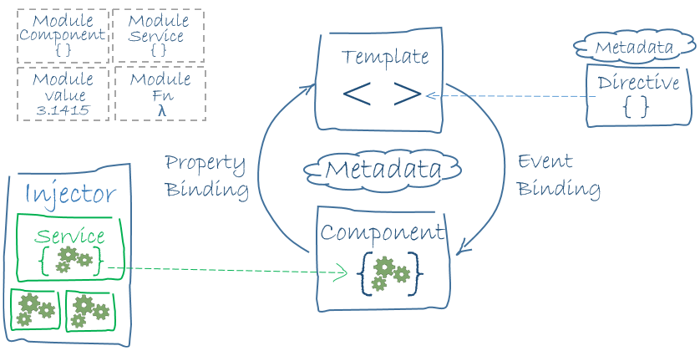
\includegraphics[width=1.0\linewidth]{angular_architecture}
	\caption{Štruktúra modulu v Angulare\cite{angular}}
	\label{angular_architecture}
\end{figure}

\subsection{Komponenty}
Na nasledujúcej ukážke kódu môžeme vidieť, ako sa dáta z komponentu (ukážka \ref{ts_snippet}) dostanú do template (ukážka \ref{html_snippet}) a opačne. Tento proces sa všeobecne nazýva \textit{binding} a v Angulare poznáme štyri typy bindingu (pozri aj Obr. \ref{angular_architecture})
\begin{description}
\item[interpolation] - vkladáme hodnotu do elementu pomocou $\{\{\}\}$, v template vidíme na riadku 3
\item[property binding] - posúvame objekt do komponentu pomocou $[ ]$, v template vidíme na riadku 4. Väčšinou ho vieme nahradiť pomocou interpolation, napríklad nastavenie vstupu children na riadku 4 v template môžeme zapísať aj ako\\
\texttt{children="\{\{user.children\}\}"}, ale z dôvodu čitateľnosti kódu je vhodné tieto dva typy nezamieňať.
\item[event binding] - volá metódu komponentu na základe udalosti pomocou $()$, v template vidíme na riadku 2
\item[two-way binding] alebo obojsmerný binding - vzniká kombináciou property bindingu a event bindingu, zapisuje sa ako $[( )]$ a využíva sa napríklad vo formulárových komponentoch, kedy môže byť hodnota ovplyvnená nie len užívateľom, ale aj inou aplikačnou logikou a je potrebné túto zmenu užívateľovi zároveň aj zobraziť.
\end{description}

\begin{lstlisting}[language=HTML,caption={HTML template \textit{user-detail.html}},captionpos=b,label=html_snippet]
<div>User Details</div>
<div (click)="callClickMethod()">
  <label>Name: {{ user.name }}</label>
  <children-list [children]="user.children"></children-list>
</div>
\end{lstlisting}

\begin{lstlisting}[caption={Komponent UserDetail},captionpos=b,label=ts_snippet]
@Component({
  selector: 'user-detail',
  templateUrl: './user-detail.html',
})
export class UserDetailComponent implements OnInit {

  public user: User;

  constructor(private _userService: UserService) { }

  ngOnInit(): void {
    this.user = this._userService.getUser();
  }
  
  public callClickMethod(): {
    console.log('clicked on detail');
  }
}
\end{lstlisting}

Na riadku 9 v ukážke \ref{ts_snippet} si zase všimneme, ako využívame zdieľanú službu, ktorá nám na riadku 12 poskytne dáta o užívateľovi. Viac informácií o zdieľaných službách sa nachádza v podkapitole \ref{sec_di}.

\subsection{Direktívy}
V prípade komponentov zvyčajne definujeme selektor, ktorý je unikátny identifikátor komponentu vrámci modulu a používa sa v template. V ukážke \ref{ts_snippet} sme tak urobili na riadku 2, čím sme umožnili použitie tohto komponentu v inom komponente zadaním HTML tagu \texttt{<user-detail></user-detail>} do template.

Direktívy umožňujú rozšírenú manipuláciu DOM objektov tak, že sa vkladajú do HTML tagov. Poznáme dva typy direktív\cite{angular}:
\begin{enumerate}
\item structural - dokážu ovplyvňovať výsledný layout odstraňovaním a pridávaním DOM objektov, napríklad vstavané direktívy *ngFor, *ngIf
\item attribute - dokážu len upravovať vlastnosti DOM objektu, napríklad vstavané direktívy *ngClass, *ngStyle
\end{enumerate}

\begin{quote}
\textit{\textbf{DOM - Document Object Model} je objektovo-orientovaná reprezentácia HTML dokumentu. Reprezentuje HTML dokument ako strom objektov s vlastnosťami (veľkosť, štýly, a pod.) a umožňuje tým JavaScriptu identifikovať, meniť, pridávať a odoberať uzly v tomto strome \cite{yang2009topic}. Pomocou DOM je teda možné dynamicky meniť obsah stránok, čo je vo svojej podstate význam JavaScriptu.}
\end{quote}

Nasledujúca jednoduchá ukážka \ref{directive_snippet} nám pomôže porozumieť správaniu direktív:
\begin{figure}
 \centering
 \begin{minipage}{.59\textwidth}

  \centering
  \begin{lstlisting}[language=HTML,caption={Direktívy použité v template (vľavo) a ako ich vo výsledku vníma prehliadač (vpravo)},label=directive_snippet]
<div *ngIf="true">I am</div>
<div *ngIf="false">I am not</div>

<div *ngFor="let i of [1,2]">
  {{ i }}
</div>
<div [style.color]="data.color">
  {{ data.color }}
</div>
  \end{lstlisting}

 \end{minipage}
 \begin{minipage}{.39\textwidth}

  \centering
  \begin{lstlisting}[language=HTML,numbers=none,xleftmargin=0em]
<div>True</div>
<!--DOM not present-->

<div>1</div>
<div>2</div>

<div style="color:red">
  <@\textcolor{red}{red}@>
</div>
  \end{lstlisting}
 
 \end{minipage}
\end{figure}

Na riadku 2 môžeme vidieť, že DOM daného divu vo výsledku vôbec nie je prítomný. Avšak v momente, kedy by sa výsledok logického výrazu vloženého do direktívy *ngIf zmenil, DOM sa aktualizuje, vytvorí sa nový objekt a prehliadač daný element vyrenderuje. Direktíva *ngIf tak patrí do prvej skupiny direktív, pretože dokáže pridávať a odoberať DOM objekty zo stránky (rovnako direktíva *ngFor na riadku 4).

Opačným príkladom je direktíva *ngStyle, ktorá v DOM mení len atribúty. V príklade na riadku 7 predpokladáme, že v komponente existuje objekt \textit{data}, ktorého atribút \textit{color} typu \texttt{string} obsahuje hodnotu "red".

\subsection{Dependency Injection}
\label{sec_di}
Dependency Injection je implementácia dizajnového vzoru IoC\footnote{IoC - Inversion of Control, prvý krát definoval Michael Mattson v roku 1996~\cite{mattsson1996object}} ktorej úlohou je zbavovať komponenty systému priamych závislostí. Cieľom je túto závislosť (dependency) implementovať samostatne ako službu a potom v danom závislom komponente vykonať injection (vloženie služby), ktorým sa komponentu umožní túto službu využiť \cite{chiba2005aspect, yang2008empirical}.

Komponent sa tým pádom nestará o vytvorenie samotného objektu, ale dostane už hotový objekt, čím sa zbavuje závislosti (na rozdiel od využívania statických metód alebo vytvárania nových objektov pomocou kľúčového slova \textit{new}).

Framework Angular umožňuje vytvárať inštancie služieb (services) pri bootstrape aplikácie. Bootstrap je jeden z procesov spúšťania, ktorý výslednú aplikáciu vloží do súboru \textit{index.html} \cite{angular} (netreba si mýliť s knižnicou Twitter Bootstrap, ktorá obsahuje HTML a CSS šablóny pre tvorbu responzívnych web stránok \cite{peska2017thesis}). Takto inicializované služby potom vieme využívať naprieč modulmi tak, ako je to znázornené v ukážke \ref{ts_snippet} na strane \pageref{ts_snippet}.

\chapter{Návrh modulu}
%Cieľom tejto práce je vytvoriť modul vo frameworku Angular, ktorý bude nasaditeľný ako samostatný portlet do Liferay portálu a prostredníctvom ktorého bude užívateľ schopný zvoliť si podmnožinu časového ohraničenia.

Kybernetický polygón generuje počas experimentu obrovské množstvo dát. Tieto dáta sa zaznamenávajú do prislúchajúcich časových postupností, z ktorých sa vytvárajú rôznorodé vizualizácie, ktoré umožňujú užívateľovi vnímať tieto dáta z viacerých pohľadov. Príklad takejto vizualizácie môžeme vidieť na obrázku \ref{visualization}.

\begin{figure}
	\center
	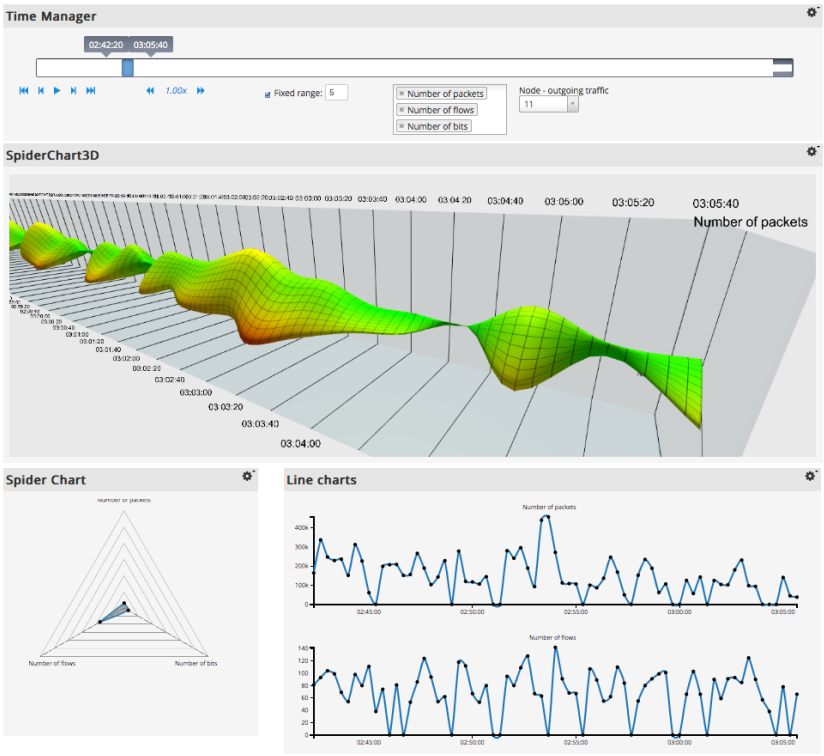
\includegraphics[width=1.0\linewidth]{visualization}
	\caption{Ukážka vizualizácií\cite{eichler2014analytical}}
	\label{visualization}
\end{figure}

Úlohou modulu interaktívnej časovej osy je poskytnúť užívateľovi intuitívny nástroj, ktorým dokáže z množstva týchto dát vybrať len určitý časový úsek a následne túto informáciu podať všetkým prislúchajúcim portletom na danej stránke. Zároveň bude tento modul spĺňať veľmi špecifické nároky na funkcionalitu, ktorým je venovaná táto kapitola. Jedným z najdôležitejších faktorov je, že celkové možné časové ohraničenie sa môže dynamicky meniť.

\section{Vstupy a Výstupy}
Vstupom tohto modulu bude
\begin{description}
\item[krok (step)] - najmenšia uvažovaná časová jednotka (získa sa volaním REST rozhrania)
\item[minimum, maximum] - dolné a horné časové ohraničenie (získa sa volaním REST rozhrania)
\item[IP adresa] na ktorú budú prebiehať REST volania z predchádzajúcich dvoch bodov (získa sa z konfigurácie portletu)
\item[perióda] - číselná hodnota v sekundách, ktorá udáva, ako často sa má cez REST znovu overiť časové ohraničenie
\begin{itemize}
\item ak je perióda nulová, periodické volania sa nevykonávajú a možné časové ohraničenie sa zistí jednorázovo
\end{itemize}
\end{description}
Výstupom tohto modulu budú dve časové známky, kde prvá odpovedá aktuálnej pozícii ľavého manipulátora a druhá pozícii pravého manipulátora.

\section{Požiadavky}
\label{requirements}
Požiadavky na dizajn a funkcionalitu som vytvoril na základe konzultácií s vedúcim práce RNDr. Radkom Ošlejškom, Ph.D.

\subsection{Funkčné požiadavky}
\label{funkcne_poziadavky}
Medzi funkčné požiadavky patria
\begin{itemize}
\item Užívateľ si na časovej ose bude môcť zvoliť časový interval, pričom tento interval bude len vrámci povolených hodnôt.
\item Užívateľ bude schopný z modulu ľahko vyčítať informáciu o práve zvolenom časovom intervale a rovnako aj o rozsahu povolených hodnôt. Ak sa jeho aktivity nezameriavajú na časový interval ale jeden konkrétny okamih, užívateľ vie zvolený okamih taktiež ľahko určiť.
\item V prípade, že možné ohraničenie sa bude dynamicky meniť, užívateľ bude vedieť definovať, ako a či vôbec sa pri zmene možného ohraničenia zmení zvolený časový interval.
\item Užívateľ bude informovaný vhodným chybovým hlásením, pokiaľ nastane chyba pri zisťovaní možného časového ohraničenia.
\end{itemize}

\subsection{Nefunkčné požiadavky}
Medzi nefunkčné požiadavky patria
\begin{itemize}
\item Modul bude pracovať s časovými známkami (timestamp), ktoré sú univerzálnym označením časového okamihu v UNIXových operačných systémoch. Výsledný modul tak nebude zohľadňovať časové pásma.
\item Modul bude implementovaný v aktuálnej verzii frameworku Angular, v dobe implementácie sa jedná o verziu \angular_version .
\item Graficky bude modul prezentovaný ako dve časové osy. Maximum spodnej časovej osy bude vždy odpovedať hornému zvolenému časovému intervalu, analogicky minimum (bude odpovedať dolnému zvolenému časovému intervalu). Vrchná časová os bude vždy reflektovať zvolený časový interval ako \textit{"spojitú"} podmnožinu možného ohraničenia. Jediným účelom spodnej osy bude spresnenie zvoleného intervalu jeho zmenšením.
\item Pri manipulátoroch (jazdcoch) na vrchnej časovej osy sa budú nachádzať klikateľné ukazatele zámkov. Tieto zámky budú implementovať funkčnú požiadavku uvedenú v sekcii \ref{funkcne_poziadavky} a užívateľ pomocou nich bude definovať správanie modulu pri zmene dát. Viac informácií o zámkoch doplňuje sekcia \ref{sec:lockers}.
\item Výška portletu bude minimalizovaná, aby zaberala čo najmenšiu vertikálnu časť obrazovky.
\item Modul bude responzívny do takej miery, že pri počiatočnom vyrenderovaní sa prispôsobí šírke samotného portletu. Šírka modulu a zobrazené dáta budú optimalizované pre najčastejšie veľkosti displejov používaných na stolných počítačoch.
\item hlavná logika modulu bude pokrytá jednotkovými testami, viac informácií o testoch sa nachádza v sekcii \ref{sec:tests}.
\begin{quote}
\textit{Pod pojmom \textbf{hlavná logika modulu} rozumieme vzťah a reagovanie na zmeny medzi týmito prvkami modulu: \textbf{pravý zámok}, \textbf{ľavý zámok}, \textbf{maximum} (je maximálna hodnota, ktorú je možné zvoliť na časovej ose), \textbf{minimum} (je minimálne hodnota, ktorú je možné zvoliť na časovej ose), \textbf{dolné zvolené ohraničenie} (pozícia ľavého manipulátora) a \textbf{horné zvolené ohraničenie} (pozícia pravého manipulátora).}
\end{quote}

\end{itemize}

\subsection{Funkcia zámkov}
\label{sec:lockers}
V prípade, že modul časovej osy bude pracovať s dátami v reálnom čase, horné ohraničenie sa logicky bude zväčšovať. V takomto prípade môžu nastať aj zmeny aktuálneho výberu, ktoré môžu ale nemusia byť pre užívateľa žiadúce.

Z tohto dôvodu vznikla už v minulosti požiadavka, aby sám používateľ portálu mal možnosť toto správanie definovať. Za týmto účelom bude pri oboch manipulátoroch vrchnej časovej osy klikateľný ukazateľ zámku, ktorého správanie opisuje nasledujúca tabuľka možností:
\begin{center}
  \begin{tabular}{ | c | c || p{6.5cm} | }
    \hline
    ľavý zámok & pravý zámok & správanie pri zmene horného ohraničenia \\ \hline \hline
    odomknutý & odomknutý & výber sa nemení, aktualizuje sa len možné horné ohraničenie viditeľné v hornej osy \\ \hline
    odomknutý & zamknutý & pravý manipulátor sa nastaví na maximum a ľavý sa posunie doprava tak, aby veľkosť zvoleného rozmedzia ostala zachovaná\\ \hline
    zamknutý & odomknutý & zakázaný stav - ľavý zámok môže byť aktivovaný len ak je aktivovaný zároveň aj pravý \\ \hline
    zamknutý & zamknutý & pravý manipulátor sa nastaví na maximum a ľavý zostáva, veľkosť zvoleného rozmedzia sa zväčší \\ \hline
  \end{tabular}
\end{center}

\subsection{Rozsah testov}
\label{sec:tests}
Modul časovej osy má na prvý pohľad jednoduchú úlohu, t.j. spresňuje časové okno vrámci povolených hodnôt. Avšak pri analýze je možné badať niekoľko rôznych vstupov a premenných ktoré sa navzájom ovplyvňujú a ovplyvňujú tak aj správanie tohto modulu, ktoré už nie je úplne triviálne.

V tejto podkapitole sa nachádza zoznam a popis jednotkových testov, ktoré testujú hlavnú logiku modulu.
\begin{enumerate}
  \item
  \begin{tabular}{ | p{2.75cm} | p{8cm} | }
    \hline
    stav pred & pravý zámok aktívny \\ \hline
    udalosť & zmení sa maximum (zväčší sa)\\ \hline
    testovaný stav & horné zvolené ohraničenie sa aktualizuje \\ \hline
  \end{tabular}

  \item
  \begin{tabular}{ | p{2.75cm} | p{8cm} | }
    \hline
    stav pred & pravý zámok nie je aktívny \\ \hline
    udalosť & zmení sa maximum (zväščí sa)\\ \hline
    testovaný stav & zvolené ohraničenie sa nezmení \\ \hline
  \end{tabular}

  \item
  \begin{tabular}{ | p{2.75cm} | p{8cm} | }
    \hline
    stav pred & pravý zámok je aktívny \\ \hline
    udalosť & horné zvolené ohraničenie sa posunie doľava (užívateľ posunie pravý manipulátor doľava)\\ \hline
    testovaný stav & pravý zámok sa deaktivuje \\ \hline
  \end{tabular}

  \item
  \begin{tabular}{ | p{2.75cm} | p{8cm} | }
    \hline
    stav pred & pravý zámok je aktívny \\ \hline
    udalosť & dolné zvolené ohraničenie sa zmení (užívateľ posunie ľavý manipulátor ľubovoľne)\\ \hline
    testovaný stav & pravý zámok ostáva aktívny a horné zvolené ohraničenie sa nezmení \\ \hline
  \end{tabular}

  \item
  \begin{tabular}{ | p{2.75cm} | p{8cm} | }
    \hline
    stav pred & ľavý zámok je aktívny \\ \hline
    udalosť & deaktivuje sa pravý zámok \\ \hline
    testovaný stav & deaktivuje sa aj ľavý zámok \\ \hline
  \end{tabular}

  \item
  \begin{tabular}{ | p{2.75cm} | p{8cm} | }
    \hline
    stav pred & pravý zámok je aktívny \\
    & ľavý zámok nie je aktívny \\ \hline
    udalosť & zmení sa maximum \\ \hline
    testovaný stav & horné aj dolné zvolené ohraničenie sa posunie doprava na maximum, zvolený interval ostane rovnako veľký \\ \hline
  \end{tabular}

  \item
  \begin{tabular}{ | p{2.75cm} | p{8cm} | }
    \hline
    stav pred & ľavý zámok je aktívny \\ \hline
    udalosť & zmení sa maximum \\ \hline
    testovaný stav & horné zvolené ohraničenie sa zmení a dolné zvolené ohraničenie sa nezmení, takže zvolený interval sa zväčší \\ \hline
  \end{tabular}
  
    \item
  \begin{tabular}{ | p{2.75cm} | p{8cm} | }
    \hline
    stav pred & pravý zámok nie je aktívny \\ \hline
    udalosť & aktivuje sa pravý zámok \\ \hline
    testovaný stav & horné zvolené ohraničenie sa nastaví na maximum \\ \hline
  \end{tabular}

    \item
  \begin{tabular}{ | p{2.75cm} | p{8cm} | }
    \hline
    stav pred & pravý zámok nie je aktívny \\ \hline
    udalosť & minimum sa zväčší alebo maximum sa zmenší\\ \hline
    testovaný stav & tento stav by logicky nemal nastať, ale ak nastane, zvolený časový interval sa nastaví tak, aby bol podmnožinou nového intervalu (aby sa manipulátory neocitli mimo osy) \\ \hline
  \end{tabular}

    \item
  \begin{tabular}{ | p{2.75cm} | p{8cm} | }
    \hline
    stav pred & pravý zámok je aktívny \\
    & ľavý zámok nie je aktívny \\ \hline
    udalosť \& testovaný stav & rovnako ako v testovacom prípade č.9\\ \hline
  \end{tabular}

\end{enumerate}

\section{Existujúce riešenie}
Existujúci portlet časovej osy pre KYPO bol implementovaný v JavaScripte vrámci diplomovej práce Jiřího Dočkala\cite{dockal2016webovy}. Okrem výberu časového ohraničenia slúžil aj na prehrávanie scenárov, ako je možné vidieť aj na Obr. \ref{old_portlet}.

V aktuálnych víziách vývojového centra KYPO sa však zrodila požiadavka na odlišný portlet, ktorý bude obsahovať v určitom smere menej funkcionality a bude postavený na odlišnej technológii (použitie frameworku Angular). Všetky tieto požiadavky boli zhrnuté v kapitole \ref{requirements}.
\begin{figure}[H]
	\center
	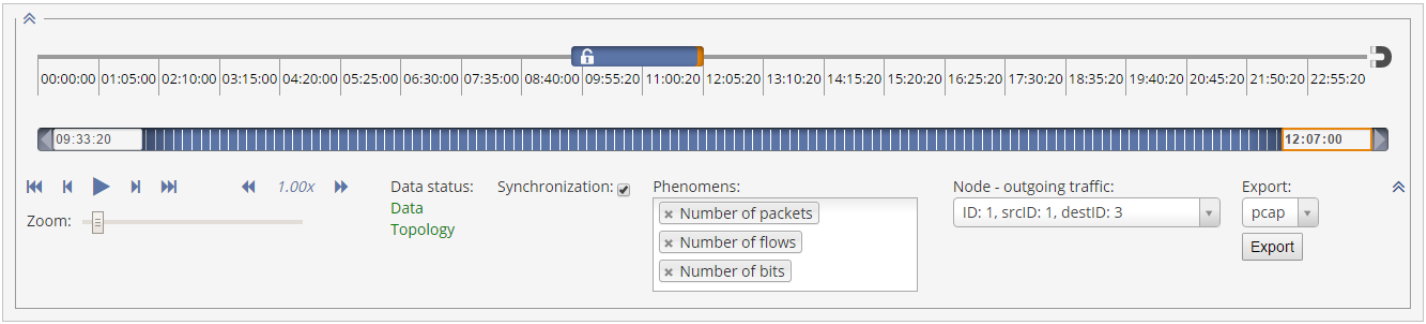
\includegraphics[width=1.0\linewidth]{old_portlet}
	\caption{Dizajn pôvodného portletu\cite{dockal2016webovy}}
	\label{old_portlet}
\end{figure}

\chapter{Implementácia}
Táto kapitola podrobne opisuje štruktúru a implementáciu modulu časovej osy, pričom berie do úvahy všetky požiadavky definované v kapitole \ref{requirements}.

\section{Výber vhodného grafického prvku}
Kľúčovou úlohou v raných fázach vývoja bolo zvoliť vhodný prostriedok, ktorým bude možné manipulovať s časovým ohraničením, resp. s časovou osou. Požiadavky sú v tomto smere pomerne jasné a najbližšie k nim je spomedzi všetkých formulárových prvkov jednoznačne \textit{range} (v preklade \textit{rozsah}, môže byť označený aj ako \textit{range slider}). Na obrázku \ref{html_range} môžeme vidieť názornú ukážku, ako takýto ovládací prvok môže vyzerať.
\begin{figure}[H]
	\center
	
\includegraphics{html_range}
	\caption{HTML prvok \texttt{<input type=\char`\"range\char`\"/>} v prehliadači Chrome a jeho prednastavený vzhľad}
	\label{html_range}
\end{figure}

Formulárový prvok typu range sa skladá z koľajnice a jazdca (manipulátora) (\ref{html_range}) a plní pre používateľa rovnakú funkciu ako bežný číselný vstup, ktorý sa zadáva do políčka prostredníctvom klávesnice, t.j. umožňuje užívateľovi zadať číselnú hodnotu. Oproti tomu má niekoľko vlastností, ktoré sú pre nás prínosom:
\begin{enumerate}
\item umožní užívateľovi vybrať číslo striktne len z daného rozsahu, čím odpadá nutnosť dodatočnej validácie (či je číslo v danom rozsahu)
\item neumožní užívateľovi zadávať nečíselné znaky, čím odpadá nutnosť ďalšej validácie (či je číslo platné)
\item užívateľ má pred sebou grafickú informáciu, kde približne sa svojou hodnotou nachádza vrámci povoleného rozsahu, čo je výhodou hlavne pri veľkých číslach.
\end{enumerate}

Medzi nevýhody formulárového prvku typu range patria:
\begin{enumerate}
\item nedá sa pohodlne ovládať len klávesnicou, vyžaduje použitie myši alebo touchpadu (pri dotykových obrazovkách dotyk a následné potiahnutie)
\item zvolená hodnota nemusí byť presná
\begin{quote}
\textit{Predstavme si, že pomocou range potrebujeme zadať hodnotu 726,54 ktorá musí byť v rozmedzí 0 až 10\,000. Trafiť sa do tejto hodnoty sa nám vôbec nemusí podariť.}
\end{quote}
\end{enumerate}

Obe spomínané nevýhody sa nás veľmi netýkajú, nakoľko:
\begin{itemize}
\item je veľmi malá pravdepodobnosť, že KYPO portál a všeobecne web bude navštevovať používateľ pracujúci výhradne s klávesnicou
\item z dôvodu nepresnosti tohto formulárového prvku je už vo funkčných požiadavkách definované, že za účelom spresnenia výberu sa bude pod hlavnou časovou osou nachádzať ešte jedna detailnejšia.
\end{itemize}

Pomocou CSS je možné vo viacerých moderných prehliadačoch upraviť prednastavený vzhľad prvku \texttt{<input type=\char`\"range\char`\">}, ale takýto prvok je pre nás stále nepoužiteľný, nakoľko okrem zopár grafických úprav nedokážeme tento prvok vôbec modifikovať. Z funkčných požiadaviek napríklad vyplýva, že na koľajnici by sa mali nachádzať dva manipulátory, keďže výsledkom (nášho výberu) nie je jedna hodnota, ale rozsah hodnôt.

\subsection{Existujúce implementácie range slidera}
Spočiatku som sa snažil využiť niekoľko už existujúcich voľne prístupných knižníc (komponent), ktoré riešili implementáciu \textit{range slider}a pre Angular (verzie 2 a vyššej). Väčšina z nich podporovala niekoľko jazdcov na koľajnici a dali sa na nich pomerne jednoducho prepisovať štýly.

Najviac času som strávil s komponentom ng2-nouislider\cite{ng2nouislider}, ale postupom času mi ani tento komponent neponúkol také možnosti, ktoré by som potreboval. Všetky knižnice mali z môjho pohľadu tieto dva nedostatky:
\begin{description}
\item[neboli pôvodne navrhnuté pre Angular] - väčšina knižníc spolupracovala s Angularom len preto, že niekto \char`\"obalil\char`\" jej existujúceho JavaScriptového predchodcu ako Angular2 komponent, čím plnohodnotne nevyužil všetky možnosti Angularu (ako napríklad obojsmerný binding)
\item[neboli navrhnuté pre tento typ použitia] - boli navrhnuté tak, aby na začiatku boli definované hraničné body (minimum, maximum) a následne po celý zvyšok svojej životnosti už len poskytovali informácie o momentálnej voľbe užívateľa. Ak sa následne zmenili hraničné body, väčšina komponent v lepšom prípade dané hranice len neaktualizovala, v horšom prípade úplne prestala fungovať.
\end{description}

\section{D3.js}
Táto JavaScriptová knižnica slúži na dynamické vizualizácie dát v prehliadačoch. Hlavnou technológiou, na ktorej je postavená táto knižnica, je vektorová grafika a konkrétne značkovací jazyk SVG.

SVG alebo Scalable Vector Graphics bol vyvynutý na opis dvojrozmernej statickej aj animovanej grafiky a využíva pritom syntax XML\cite{quint2003scalable}.
Dnes je SVG formát široko podporovaný väčšinou webových prehliadačov. Je možné vkladať ho priamo do HTML kódu a následne interpretovať. SVG má oproti štandardným rastrovým obrázkom hneď niekoľko výhod, z nich najpodstatnejšie pre webový vývoj sú tieto:
\begin{itemize}
\item SVG obrázky sú škálovateľné. Vyplýva to z predpokladu, že hovoríme o vektorovej grafike. Pri rôznych veľkostiach toho istého obrázka nestrácame žiadnu informáciu. Hlavne v oblasti responzívneho dizajnu je to veľmi podstatný faktor.
\item Veľkosť - keďže sa jedná o textovú informáciu, výsledný súbor je veľmi malý. Navyše nám pre viacero rozlíšení postačuje jeden a ten istý a nepotrebujeme vytvárať viacero obrázkov pre rôzne veľkosti. Tento faktor je podstatný hlavne v oblasti mobilného vývoja, kde je jednou z požiadaviek aj veľkosť prenášaných dát.
\item Ak obrázok obsahuje text, je možné ho vyhľadať a vedia ho prečítať aj roboty vyhľadávačov, čo je pri weboch veľké plus.
\end{itemize}

D3.js umožňuje pridávať do DOMu stránky SVG elementy. Týmto spôsobom vieme "programovať", ako sa má grafika zobraziť a odchytávať rôzne typy udalostí ako sú napríklad kliknutia. Toto je hlavný princíp, na ktorom je postavená implementácia modulu.

Implementoval som direktívy, ktoré majú niekoľko vstupov, ako napríklad minimum, maximum, zvolený časový úsek a podobne. Na základe týchto informácií direktíva vytvorí SVG element, v ktorom vykreslí koľajnicu a dvoch jazdcov (manipulátory). Udalosť kliknutia a ťahania týchto jazdcov odchytávam a pomocou nich viem upraviť výsledný časový úsek aj vzhľad.

Vo výsledku teda môžeme povedať, že dve časové osy, ktoré vidíme v tomto module, sú v podstate dva vektorové obrázky.

\section{Ikony Font-Awesome}
Vzhľad modulu 

\section{Technológie}
Vrámci nefunkčných požiadaviek bol pre implementáciu zvolený framework Angular od Google, ktorého verzia v čase tvorby tejto práce bola \angular_version . Tento framework bol v prostredí KYPO zvolený globálne a preto je táto voľba logická.


%\printbibliography

\printbibliography[heading=bibintoc] %% Print the bibliography.

  \makeatletter\thesis@blocks@clear\makeatother
  \phantomsection %% Print the index and insert it into the
  \addcontentsline{toc}{chapter}{\indexname} %% table of contents.
  \printindex

\appendix %% Start the appendices.
\chapter{An appendix}
Here you can insert the appendices of your thesis.

\end{document}